\section{Results}
\label{sec:results}

\subsection{Experiment~A: the Engineered Task at 20 Qubits}
\label{sec:results_a}

\Tabref{tab:exp_a_headline} reports the headline comparison at $n=20$ qubits
(seed $0$), averaged over $10$ stratified splits. The projected quantum kernel
\pqk{} reaches $0.865 \pm 0.043$ test accuracy, while the best classical model
(gradient boosting) reaches $0.629 \pm 0.035$. Every classical model except the
two tree ensembles sits at or below chance, and the cross-validated RBF-SVM---the
canonical kernel to beat---reaches only $0.489$. The paired $t$-test of \pqk{}
against the best classical model gives $t=16.95$, $p=3.9\times10^{-8}$, Cohen's
$d=5.36$, and a mean gap of $+0.236$, far past the pre-registered thresholds of
$\Delta>0.2$ and $p<0.05$ (\figref{fig:bars}).

\begin{table}[t]
    \centering
    \caption{\textbf{Experiment~A, engineered task at $n=20$ qubits (seed $0$).}
    Test and train accuracy (mean $\pm$ std over $10$ stratified splits). Chance
    is $0.50$. The projected quantum kernel generalizes; the fidelity quantum
    kernel concentrates to chance despite perfect train accuracy, exactly like the
    over-parameterized classical models. Best test result in \textbf{bold}.}
    \label{tab:exp_a_headline}
    \begin{tabular}{@{}lccl@{}}
        \toprule
        \textbf{Model} & \textbf{Test acc.} & \textbf{Train acc.} & \textbf{Note} \\
        \midrule
        \textbf{Quantum: Projected kernel} & \textbf{0.865} {\scriptsize $\pm$ 0.043} & 1.000 & generalizes \\
        \midrule
        Classical: Gradient Boosting & 0.629 {\scriptsize $\pm$ 0.035} & 1.000 & best classical \\
        Classical: Random Forest & 0.607 {\scriptsize $\pm$ 0.046} & 1.000 & \\
        Classical: Logistic Reg. & 0.496 {\scriptsize $\pm$ 0.046} & 0.639 & chance \\
        Quantum: \emph{Fidelity} kernel & 0.493 {\scriptsize $\pm$ 0.000} & 1.000 & concentrates $\to$ chance \\
        Classical: Linear-SVM & 0.489 {\scriptsize $\pm$ 0.051} & 0.650 & chance \\
        Classical: RBF-SVM (tuned) & 0.489 {\scriptsize $\pm$ 0.029} & 0.798 & chance \\
        Classical: RBF kernel (precomp.) & 0.479 {\scriptsize $\pm$ 0.055} & 0.789 & chance \\
        Classical: MLP & 0.436 {\scriptsize $\pm$ 0.045} & 1.000 & overfits below chance \\
        \bottomrule
    \end{tabular}
\end{table}


\begin{figure}[t]
    \centering
    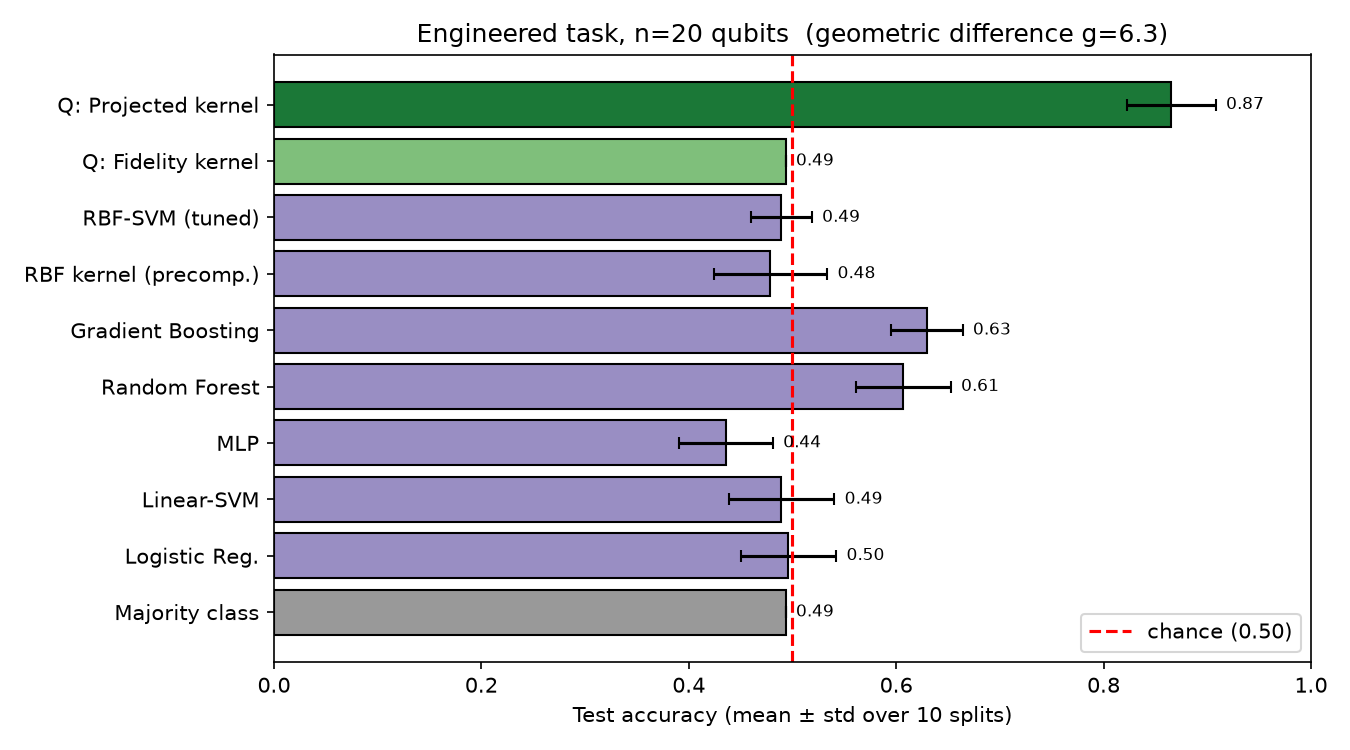
\includegraphics[width=0.7\linewidth]{figures/fig1_engineered_n20_bars.png}
    \caption{\textbf{Engineered task at $n=20$ qubits.} Test accuracy of the
    projected quantum kernel against the full classical suite and the fidelity
    control. The projected kernel ($0.865$) is the only model far above chance
    (dashed line); the fidelity kernel and the tuned RBF-SVM both sit at chance.}
    \label{fig:bars}
\end{figure}

\para{The fidelity kernel collapses---the win is the \emph{right} kernel.} The
within-quantum control is decisive. At 20 qubits the naive fidelity kernel \fqk{}
attains train accuracy $1.000$ but test accuracy $0.493$---exactly chance. This is
the exponential-Hilbert-space concentration predicted by
\citet{huang2021power,kubler2021inductive}: in the $2^{20}$-dimensional space all
states become nearly orthogonal, so the kernel memorizes the training set and
generalizes at chance, just like the over-parameterized MLP (which actually drifts
\emph{below} chance to $0.436$ by overfitting noise). Only the projected kernel,
which carries a problem-matched inductive bias, wins. Quantumness alone is not
enough.

\subsection{Scaling Across Qubit Count}
\label{sec:results_scaling}

\Tabref{tab:exp_a_scaling} aggregates $3$ seeds per qubit count.
The projected-quantum advantage is \emph{stable} at $\approx 0.22$--$0.23$ across
$n=8,10,20$ (\figref{fig:scaling}). We had predicted the gap would \emph{widen}
with $n$; instead it holds steady while the geometric difference \gdiff{} shrinks
from $22.6$ to $6.2$. The honest reading: at fixed $N=250$ and fixed bandwidth the
20-qubit projected kernel concentrates somewhat (quantum accuracy drifts
$0.919\to0.854$), but classical accuracy falls in step
($0.699\to0.623$), so the gap is preserved. \gdiff{} stays $\gg 1$, so the
advantage remains available at every scale; the fidelity kernel is at chance by
$n=20$. We read this as a more conservative conclusion than the original
hypothesis: the advantage is \emph{robust} to scale rather than growing with it.

\begin{table}[t]
    \centering
    \caption{\textbf{Experiment~A, scaling across qubit count} (mean $\pm$ std over
    $3$ dataset seeds, $10$ splits each). The projected-quantum advantage $\Delta$
    is stable at $\approx 0.22$--$0.23$ from $8$ to $20$ qubits. The geometric
    difference \gdiff{} shrinks as the Hilbert space dilutes the projected
    distances but stays $\gg 1$. The fidelity kernel reaches chance by $n=20$.
    Best per-row in \textbf{bold}.}
    \label{tab:exp_a_scaling}
    \begin{tabular}{@{}cccccc@{}}
        \toprule
        $n$ \textbf{qubits} & \textbf{Projected quantum} & \textbf{Best classical} & \textbf{$\Delta$ (gap)} & \textbf{\gdiff} & \textbf{Fidelity kernel} \\
        \midrule
        $8$  & \textbf{0.919} {\scriptsize $\pm$ 0.029} & 0.699 {\scriptsize $\pm$ 0.053} & $+0.220$ & 22.6 & --- \\
        $10$ & \textbf{0.915} {\scriptsize $\pm$ 0.013} & 0.687 {\scriptsize $\pm$ 0.046} & $+0.228$ & 13.9 & --- \\
        $\mathbf{20}$ & \textbf{0.854} {\scriptsize $\pm$ 0.009} & 0.623 {\scriptsize $\pm$ 0.014} & $+0.231$ & 6.2 & 0.493 \\
        \bottomrule
    \end{tabular}
\end{table}


\begin{figure}[t]
    \centering
    \begin{subfigure}[b]{0.46\textwidth}
        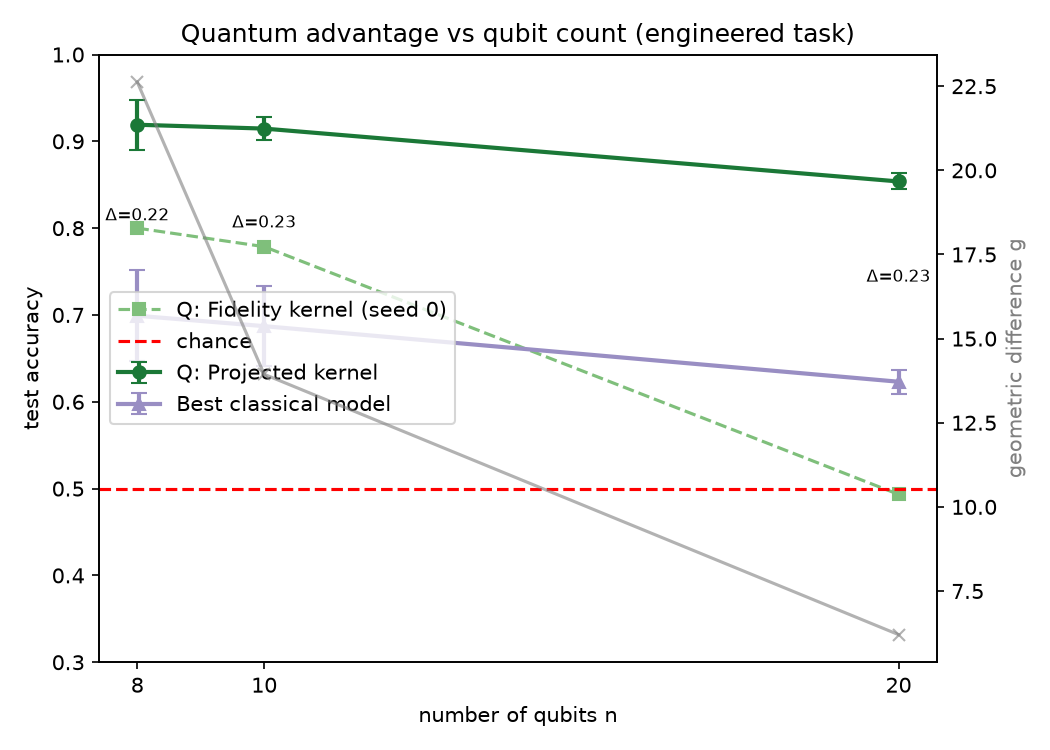
\includegraphics[width=\textwidth]{figures/fig2_accuracy_vs_qubits.png}
        \caption{Accuracy vs.\ qubit count}
        \label{fig:scaling}
    \end{subfigure}
    \hfill
    \begin{subfigure}[b]{0.46\textwidth}
        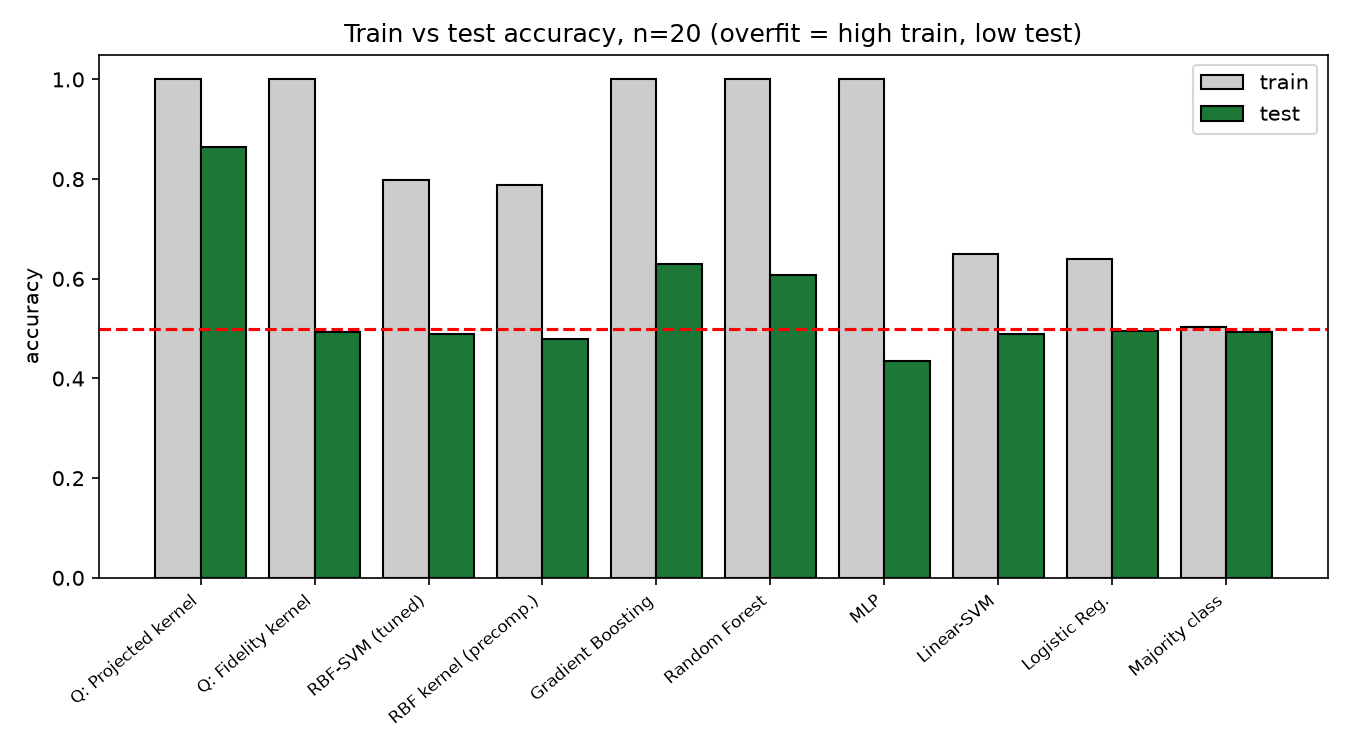
\includegraphics[width=\textwidth]{figures/fig4_generalization_gap.png}
        \caption{Generalization gap at $n=20$}
        \label{fig:gengap}
    \end{subfigure}
    \caption{\textbf{Scaling and generalization.} \captiona~The projected-quantum
    advantage holds steady at $\approx 0.22$--$0.23$ across $8$, $10$, and $20$
    qubits as both quantum and classical accuracies drift down together.
    \captionb~Train minus test accuracy at $20$ qubits: the projected kernel
    generalizes, while the fidelity kernel and over-parameterized classical models
    reach perfect train accuracy yet fail to generalize.}
    \label{fig:scaling_gap}
\end{figure}

\subsection{Experiment~B: Off-the-Shelf Classical Failure on Discrete Log}
\label{sec:results_b}

\Tabref{tab:exp_b} reports the discrete-log task across $12$/$17$/$21$ bits. Every
one of the six off-the-shelf classical models stays at chance ($0.49$--$0.52$)
while the quantum interval-state kernel \isk{} separates the task near-perfectly
($0.997 \to 1.000$ as bit size grows), with the gap flagged in advance by an
enormous geometric difference $\gdiff \approx 120$--$181$ (\figref{fig:dlog}).

\begin{table}[t]
    \centering
    \caption{\textbf{Experiment~B, discrete-log task} (test accuracy, mean $\pm$
    std over $10$ splits). Chance is $0.50$. Every off-the-shelf classical model
    stays at chance across all bit sizes while the quantum interval-state kernel
    separates the task near-perfectly. The enormous geometric difference \gdiff{}
    flags the gap before training. Best per-row in \textbf{bold}.}
    \label{tab:exp_b}
    \resizebox{\textwidth}{!}{%
    \begin{tabular}{@{}lcccc@{}}
        \toprule
        \textbf{Problem} & \textbf{Quantum interval kernel} & \textbf{Best classical} & \textbf{All classical range} & \textbf{\gdiff} \\
        \midrule
        $n=12$ bit ($p=4079$) & \textbf{0.997} {\scriptsize $\pm$ 0.003} & 0.516 (logreg) & 0.490--0.516 & 171 \\
        $n=17$ bit ($p=65543$) & \textbf{0.999} {\scriptsize $\pm$ 0.001} & 0.504 (MLP) & 0.491--0.504 & 181 \\
        $n=21$ bit ($p=1048703$) & \textbf{1.000} {\scriptsize $\pm$ 0.001} & 0.521 (linear SVM) & 0.497--0.521 & 120 \\
        \bottomrule
    \end{tabular}
    }
\end{table}


\begin{figure}[t]
    \centering
    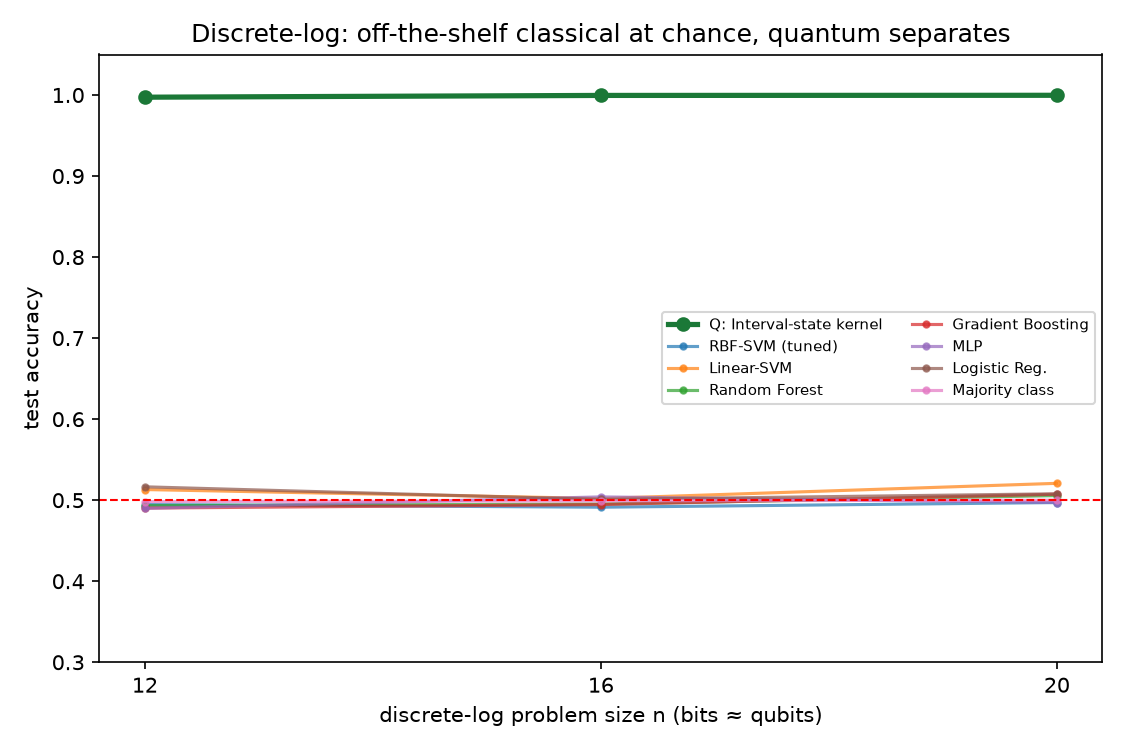
\includegraphics[width=0.7\linewidth]{figures/fig3_discrete_log.png}
    \caption{\textbf{Discrete-log task across bit sizes.} The quantum
    interval-state kernel stays near $1.0$ from $12$ to $21$ bits, while all six
    off-the-shelf classical models remain pinned at chance ($0.50$, dashed line).
    The $21$-bit problem requires $\ge 20$ qubits.}
    \label{fig:dlog}
\end{figure}

\para{Memorization without generalization.} The classical failure is not a tuning
artifact. Random forest and MLP reach train accuracy $1.000$ at every bit size yet
test at $\approx 0.50$: they \emph{memorize} the training labels but cannot
generalize, because the labels are information-theoretically random in the
bit-input space without computing the discrete log. This is the precise signature
of a representation in which the target is unlearnable, and it holds even as the
$21$-bit problem crosses the $\ge 20$-qubit threshold.
